\documentclass[12pt]{article}

\usepackage{amsmath}
\usepackage{amssymb}
\usepackage{amsthm}
\usepackage{centernot}
\usepackage{fullpage}
\usepackage{makecell}
\usepackage{tabularx}
\usepackage[hypcap=false]{caption}
\usepackage{tikz, tkz-euclide}
\usetikzlibrary{decorations.pathreplacing,arrows}
\usetikzlibrary{quotes,angles,calc,intersections}

\usepackage{titling}
\usepackage{pdfpages}
\usepackage{enumitem}
\usepackage{multicol}
\usepackage{bm}

\usepackage{linear}
\usepackage{common}

\begin{document}

\title{Abstract Algebra}
\author{Brendan Burkhart}
\maketitle

\tableofcontents
\newpage

\section{Symmetries}

Our first motivation for studying groups will be the symmetries of regular $n$-gons, starting with the regular $3$-gon: the equilateral triangle. The symmetries of a regular $n$-gon in the plane are rotations and reflections which take the $n$-gon to itself.

For example, if we take an equilateral triangle and label the vertices $A, B, C$, in anti-clockwise order starting from the top, we have two rotational symmetries: rotation by $120^\circ$ and rotation by $240^\circ$, in a particular sense or direction, say anti-clockwise. We also have three reflection symmetries -- reflections across a line going from one vertex to the midpoint of the opposite edge.

\begin{figure}[ht!]
    \centering
    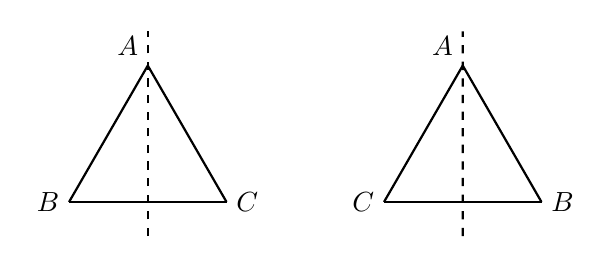
\begin{tikzpicture}
        \coordinate (A1) at (0, {sqrt(3)});
        \coordinate (B1) at (-1, 0);
        \coordinate (C1) at (1, 0);
        \coordinate (R1) at ($(B1)!0.5!(C1)$);
        \coordinate (R11) at ($(A1)!1.25!(R1)$);
        \coordinate (R12) at ($(R1)!1.25!(A1)$);

        \node[anchor=south east] at (A1) {$A$};
        \node[anchor=east] at (B1) {$B$};
        \node[anchor=west] at (C1) {$C$};

        \draw [thick] (A1)--(B1);
        \draw [thick] (B1)--(C1);
        \draw [thick] (C1)--(A1);

        \draw [thick, dashed] (R11)--(R12);

        \coordinate (A2) at (4, {sqrt(3)});
        \coordinate (B2) at (5, 0);
        \coordinate (C2) at (3, 0);
        \coordinate (R2) at ($(B2)!0.5!(C2)$);
        \coordinate (R21) at ($(A2)!1.25!(R2)$);
        \coordinate (R22) at ($(R2)!1.25!(A2)$);

        \node[anchor=south east] at (A2) {$A$};
        \node[anchor=west] at (B2) {$B$};
        \node[anchor=east] at (C2) {$C$};

        \draw [thick] (A2)--(B2);
        \draw [thick] (B2)--(C2);
        \draw [thick] (C2)--(A2);

        \draw [thick, dashed] (R21)--(R22);
    \end{tikzpicture}
\caption{Reflection symmetry $S_1$}
\label{fig:triangle-reflection}
\end{figure}

Let $R$ be the rotation by $120^\circ$ anti-clockwise. Then the rotation by $240^\circ$ anti-clockwise is simply $R$ applied twice, so we will denote it by $R^2$. Let $S_1$ be the reflection symmetry across the line through the top vertex, $S_2$ across the line through the left vertex, and $S_2$ the right vertex. The final symmetry is the identity transform, which we will call $e$. The triangle therefore has six symmetries in total: $\{e, S_1, S_2, R, R^2\}$.

\begin{figure}[ht!]
    \centering
    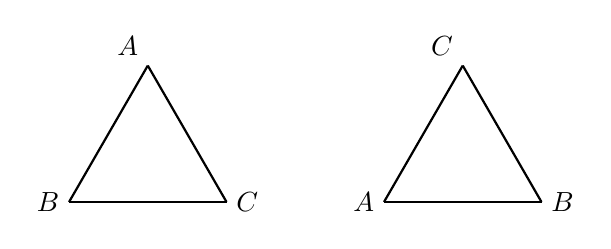
\begin{tikzpicture}
        \coordinate (A1) at (0, {sqrt(3)});
        \coordinate (B1) at (-1, 0);
        \coordinate (C1) at (1, 0);

        \node[anchor=south east] at (A1) {$A$};
        \node[anchor=east] at (B1) {$B$};
        \node[anchor=west] at (C1) {$C$};

        \draw [thick] (A1)--(B1);
        \draw [thick] (B1)--(C1);
        \draw [thick] (C1)--(A1);

        \coordinate (A2) at (3, 0);
        \coordinate (B2) at (5, 0);
        \coordinate (C2) at (4, {sqrt(3)});

        \node[anchor=east] at (A2) {$A$};
        \node[anchor=west] at (B2) {$B$};
        \node[anchor=south east] at (C2) {$C$};

        \draw [thick] (A2)--(B2);
        \draw [thick] (B2)--(C2);
        \draw [thick] (C2)--(A2);
    \end{tikzpicture}
\caption{Rotation symmetry $R$}
\label{fig:triangle-rotation}
\end{figure}

Since every symmetry takes the triangle to itself, products (compositions) of Symmetries are themselves symmetries. If $u$ and $w$ are symmetries, let $uw$ denote the composition of first $w$ and then $u$ after the manner of function composition. For example, $S_1S_2 = R$, $RR = R^2$, and $R^2R = e$.

Note that multiplication of symmetries is not necessarily commutative: $S_1S_2 = R$, but $S_2S_1 = R^2$. Multiplication with the identity is however commutative: $eR^2 = R^2 = R^2e$, etc.

We can construct a full multiplication table for the six symmetries of the $3$-gon listing all possible binary products, which is shown in Table \ref{triangle-multiplication-table}.

\begin{minipage}{\linewidth}
    \begin{center}
    \captionof{table}{Group multiplication table for $3$-gon}
    \label{triangle-multiplication-table}
    \begin{tabular}{|c||c|c|c|c|c|c|}
    \hline
    \thead{$\circ$} & \thead{$e$} & \thead{$S_1$} & \thead{$S_2$} & \thead{$S_3$} & \thead{$R$} & \thead{$R^2$}\\
    \hline\hline
    $e$   & $e$   & $S_1$ & $S_2$ & $S_3$ & $R$   & $R^2$ \\ \hline
    $S_1$ & $S_1$ & $e$   & $R$   & $R^2$ & $S_2$ & $S_3$ \\ \hline
    $S_2$ & $S_2$ & $R^2$ & $e$   & $R$   & $S_3$ & $S_1$ \\ \hline
    $S_3$ & $S_3$ & $R$   & $R^2$ & $e$   & $S_1$ & $S_2$ \\ \hline
    $R$   & $R$   & $S_3$ & $e$   & $S_2$ & $R^2$ & $e$   \\ \hline
    $R^2$ & $R^2$ & $S_2$ & $S_3$ & $S_1$ & $e$   & $R$   \\ \hline
    \end{tabular}
    \end{center}
\end{minipage}

\section{Group Axioms}

\begin{defn}
    A \emph{group} $G$ is a set together with a closed binary operation on the elements of the set (typically called ``multiplication'') that satisfies the following axioms:
    \begin{itemize}
        \item There exists an identity element $e \in G$ such that $ex = x = xe$ for every $x \in G$.
        \item Every element $x \in G$ has an inverse $x^{-1}$ such that $xx^{-1} = e$.
        \item The operation is associative: $x(yz) = (xy)z$, for every $x, y, z \in G$.
    \end{itemize}
\end{defn}

\begin{exmp}
    The symmetries of a triangle $\{e, S_1, S_2, S_3, R, R^2\}$, together with the binary operation of composition, form a group. Table \ref{triangle-multiplication-table} shows that every element has an inverse and that composition of these symmetries is closed. Associativity comes from the fact that $(xy)z$ means apply the symmetry $z$, then $y$, and then $x$, and $x(yz)$ also means apply $z$, then $y$, and then $x$, so the result is the same and $(xy)z = x(yz)$.
\end{exmp}

\begin{exmp}
    $\N$, $\Z$, $\Q$, $\R$, and $\C$ all form groups under addition, and $\Q - \{0\}$, $\R - \{0\}$, and $\C - \{0\}$ form groups under multiplication.
\end{exmp}

\begin{exmp}
    $\{1, -1, i, -i\} \subset \C$ forms a group under complex multiplication. It can be easily verified it is closed under multiplication, $1$ is the identity, and it inherits associativity from $\C$. Inverse can be easily checked: $(-1)(-1) = 1$ and $i(-i) = 1$.
\end{exmp}

\begin{defn}
    If a group is commutative, then it is an \emph{abelian} group.
\end{defn}

\begin{defn}
    The \emph{order} of a group is the cardinality of the group.
\end{defn}

\begin{defn}
    A \emph{subgroup} $H$ of a group $G$ is a set $H \subseteq G$ that forms a group under the same group operation as $G$. If $H$ is a subgroup of $G$ this may be denoted by $H \leqslant G$, or $H < G$ if it is a strict subgroup.
\end{defn}

\begin{thm}
    A non-empty subset $H$ of a group $G$ is a subgroup of $G$ if and only if $x, y \in H$ implies $xy^{-1} \in H$.
\end{thm}

\begin{proof}\proofbreak
    ($\implies$) If $H$ is a subgroup of $G$, then since $y \in H$ it must be that $y^{-1} \in H$. Since groups are closed under the group operation, $x, y^{-1} \in H$ then implies that $xy^{-1} \in H$.

    ($\impliedby$) Since $H$ is non-empty, there must exist some $x \in H$, and so $xx^{-1} \in H$, which implies $H$ contains the identity. $H$ clearly inherits associativity from $G$, so it only remains to check that it contains inverses and is closed. Since $e, x \in H$, $ex^{-1} \in H$, but $ex^{-1} = x$ so $H$ contains all inverses. Finally, if $x, y \in H$, we also have $x, y^{-1} \in H$, so $xy \in H$ and so $H$ is closed.
\end{proof}

\begin{thm}
    Let $H, K \subseteq G$ be subgroups. Then $H \intersection K$ is a subgroup of $G$.
\end{thm}

\begin{proof}
    Since $e \in H$ and $e \in K$, we of course have $e \in H \intersection K$. If $x \in H \intersection K$, then $x^{-1} \in H$ and $x^{-1} \in K$ so $x \in H \intersection K$. If $x, y \in H \intersection K$, then $xy \in H$ and $xy \in K$ so $xy \in H \intersection K$. Finally, $H \intersection K$ inherits associativity from $G$, so it is a subgroup.
\end{proof}

\section{Cyclic Groups}

\begin{defn}
    Let $G$ be a group, where $e \in G$ is the identity. For any $x \in G$, we define $x^0 = e$, and for $n \in \Z^+$ we define $x^n = x^{n-1}$. Finally, we define $x^{-n} = \left(x^n\right)^{-1}$.
\end{defn}

\begin{defn}
    Let $G$ be a group. If there exists some $x \in G$ such that for every $y \in G$ we have $y = x^n$ for some $n \in \Z$, then we say that $G$ is \emph{cyclic}, and that $x$ \emph{generates} $G$.
\end{defn}

\begin{defn}
    Let $G$ be a group. If there exists some $x_1, x_2, \ldots, x_k \in G$ such that for every $y \in G$ we have $y = x_1^{a_1}x_2^{a_2}{\cdots}x_k^{a_k}$ for some $a_1, a_2, \ldots, a_k \in \Z$, then we say that $G$ is generated by $\{x_1, x_2, \ldots, x_k\}$, and that $\{x_1, x_2, \ldots, x_k\}$ \emph{generates} $G$.
\end{defn}

\begin{defn}
    Let $G$ be a group, and $x$ be an element of $G$. The set of all elements of $G$ generated by $x$ may be denoted by $\langle{x}\rangle$.
\end{defn}

\begin{prop}
    Let $G$ be a group, and $x \in G$. Then $\langle{x}\rangle$ is a subgroup of $G$.
\end{prop}

\begin{proof}
    Given $x^n, x^m \in \langle{x}\rangle$, $x^nx^m = x^{n+m} \in \langle{x}\rangle$, so $\langle{x}\rangle$ is closed.

    Since $x^0 = e$, it has the identity, and since for any $x^n$ we have $x^{-n}$, and $x^{-n}x^n = x^0 = e$, $\left(x^n\right)^{-1} \in \langle{x}\rangle$. Finally, $\langle{x}\rangle$ inherits associativity from $G$.
\end{proof}

\begin{defn}
    The \emph{order} of an element $x$ is the order of $\langle{x}\rangle$.
\end{defn}

\begin{prop}
    Let $G$ be a group. Then for any $x \in G$, $x^n = e$ if and only if $x$ has finite order $n$.
\end{prop}

\begin{proof}\proofbreak
    ($\implies$) If $x^n = e$, then for any $k = qn + r$ where $q, r \in \Z$ and $0 \leq r < n$, we know $x^k = (x^n)^qx^r = e^qx^r = x^r$, so any element $x^k \in \langle{x}\rangle$ is one of $\{x^0, x^1, \ldots, x^{n-1}\}$. It follows that the order of $x$ is $n$.

    ($\impliedby$) If $\langle{x}\rangle$ has order $n$, then it is equal to $\{x^0, x^1, \ldots, x^{n-1}\}$. Since every element has an inverse, there is some $m \leq n-1$ such that $x^1x^m = x^0 = e$, so $x^{m+1} = e$. If $m+1 < n$, then $\langle{x}\rangle$ would have order less than $n$, which is false, so $m+1 = n$, and so $x^n = e$.
\end{proof}

\begin{cor}
    Since $x^n = e$, it follows that $\left(x^m\right)^{-1} = x^{n-m}$.
\end{cor}

\begin{exmp}
    $\Z$ is cyclic, and is generated by $1$ since $n = 1 \cdot n$, as well as by $-1$.
\end{exmp}

\begin{rmk}
    If $G$ is a cyclic group that is generated by $x \in G$, then $G$ is also generated by $x^{-1}$.
\end{rmk}

\begin{exmp}
    $\Z/n\Z$ is a \emph{finite} cyclic group, and is generated by $1$ and $n-1$ (since $1^{-1} = n-1$).
\end{exmp}

\begin{prop}
    All cyclic groups are abelian.
\end{prop}

\begin{proof}
    Let $G$ be a cyclic group, and $m \in G$ such that $m$ generates $G$. Now consider any $x, y \in G$. We know that there exists some $n_1, n_2 \in \Z$ such that $x = m^{n_1}$ and $y = m^{n_2}$, so $xy = m^{n_1}m^{n_2} = m^{n_1 + n_2} = m^{n_2}m^{n_1} = yx$.
\end{proof}

\begin{lemma}\label{cyclic-subgroups-of-z}
    All subgroups of $\Z$ are cyclic.
\end{lemma}

\begin{proof}
    Let $H$ be a subgroup of $\Z$. If $H = \{0\}$, then $H$ is trivially cyclic, so assume $H \neq \{0\}$. For any $x \in H$, $-x$ must also be in $H$, and so since $H \neq \{0\}$ there must be some smallest positive integer $m$ in $H$.

    Now consider any $k \in H$. We know that $k = qm + r$ for some $q \in \Z$ and $0 \leq r < m$ -- that is, $r = k \bmod m$ and $q = \frac{k - r}{m}$. Since $m, k \in H$, and $r = k + (-qm)$, we know that $r \in H$. Since $m$ is the smallest positive integer in $H$, it follows that $r = 0$. Therefore, $k = qm$, so $m$ generates all of $H$, and it follows that $H$ must be cyclic.
\end{proof}

\begin{thm}
    Let $G$ be a cyclic group, and $H$ a subgroup of $G$. Then $H$ is itself cyclic.
\end{thm}

\begin{proof}
    Let $x$ be any generating element of $G$. We know that for any $y \in H$, there exists some $n \in \Z$ such that $y = x^n$. Consider \[K = \left\{n \in \Z \compbar x^n \in H\right\}.\] We can show that $K$ is a subgroup of $\Z$: if $n_1, n_2 \in K$, then $x^{n_1}x^{n_2} = x^{n_1 + n_2} \in H$, so $n_1 + n_2 \in K$, so $K$ is closed. Since $x^0 \in H$, $K$ has the identity, and since $x^{-n} \in H$, we have $n \in K$ for any $n \in K$. Finally, $K$ inherits associativity from $\Z$. By Lemma \ref{cyclic-subgroups-of-z}, it follows that $K$ is cyclic.

    Since $K$ is cyclic, it is generated by some $m \in K$. Therefore, every $y \in H$ can be expressed as $x^{qm}$ for some $q \in \Z$, and so $y = (x^m)^q$. It follows that $H$ is generated by $x^m$, and so $H$ is cyclic.
\end{proof}

\section{Permutations}

\begin{defn}
    Let $X$ be a set, and let $S_X$ be the set of all bijections from $X$ to itself. These bijections are called \emph{permutations} of $X$.
\end{defn}

\begin{prop}
    For a given set $X$, $S_X$ is a group.
\end{prop}

\begin{proof}
    Composition of bijections is of course a bijection, so $S_X$ is closed. Since the inverse of a bijection is also a bijection, $S_X$ has inverses, and of course the identity function is then the identity of $S_X$. Finally, composition of functions is associative so $S_X$ is a group.
\end{proof}

\begin{defn}
    For $n \in Z^+$, the finite \emph{symmetric group} $S_n$ is the group $S_X$ where $X = \{1, 2, \ldots, n\}$.
\end{defn}

\begin{rmk}
    $S_n$ has order $n!$.
\end{rmk}

\begin{rmk}
    We may denote permutations in the form
    $\begin{bmatrix}
        a & b & c \\ c & b & a
    \end{bmatrix}$, meaning $a$ is sent to $c$, $b$ is sent to $b$, and $c$ is sent to $a$.
\end{rmk}

\begin{exmp}
    \[S_3 = \left\{
        \begin{bmatrix}
            1 & 2 & 3 \\ 1 & 2 & 3
        \end{bmatrix},
        \begin{bmatrix}
            1 & 2 & 3 \\ 1 & 3 & 2
        \end{bmatrix},
        \begin{bmatrix}
            1 & 2 & 3 \\ 2 & 1 & 3
        \end{bmatrix},
        \begin{bmatrix}
            1 & 2 & 3 \\ 2 & 3 & 1
        \end{bmatrix},
        \begin{bmatrix}
            1 & 2 & 3 \\ 3 & 1 & 2
        \end{bmatrix},
        \begin{bmatrix}
            1 & 2 & 3 \\ 3 & 2 & 1
        \end{bmatrix}
    \right\}\]

    The composition
    \[\begin{bmatrix}
        1 & 2 & 3 \\ 2 & 3 & 1
    \end{bmatrix}
    \begin{bmatrix}
        1 & 2 & 3 \\ 3 & 2 & 1
    \end{bmatrix}\] is read right to left, and so is equal to
    \[\begin{bmatrix}
        1 & 2 & 3 \\ 1 & 3 & 2
    \end{bmatrix}.\]
\end{exmp}

\begin{defn}
    The above notation for writing permutations is rather cumbersome, so \emph{cyclic notation} is commonly used. In this notation, we write $\begin{bmatrix}
        1 & 2 & 3 \\ 2 & 3 & 1
    \end{bmatrix}$ as $(123)$, meaning that $1$ is sent to $2$, $2$ is sent to $3$, and $3$ is sent back to $1$, ending the cycle. Every permutation can be written as the composition of a finite number of disjoint cycles.
\end{defn}

\begin{defn}
    A \emph{transposition} is a permutation which swaps two elements, leaving the others unchanged. It can therefore be written as $(ab)$ is cyclic notation, where $a$ and $b$ are the elements being swapped.
\end{defn}

\begin{thm}\label{transpositions-generate-sn}
    Let $X = \left\{(ab) \compbar a, b \in \{1, 2, \ldots, n\}\right\}$, the set of all transpositions in $S_n$. $S_n$ is generated by $X$.
\end{thm}

\begin{proof}
    Since any permutation in $S_n$ is the product of disjoint cycles, it is sufficient to show that any cycle is the product of (not necessarily disjoint) transpositions. Let $(a_1a_2\ldots a_k)$ be a cycle. Then
    \[(a_1a_k)(a_1a_{k-1})\cdots(a_1a_2) = (a_1a_2\ldots a_k).\]
\end{proof}

\begin{thm}\label{one-transpositions-generate-sn}
    Let $X = \left\{(1a) \compbar a \in \{1, 2, \ldots, n\}\right\}$, the set of all transpositions in $S_n$ which start with $1$. $S_n$ is generated by $X$.
\end{thm}

\begin{proof}
    By Theorem \ref{transpositions-generate-sn}, the set of transpositions in $S_n$ generate $S_n$, so we only need to show that the set of transpositions of the form $(1a) \in S_n$ can be used to create the set of transpositions in $S_n$.

    Let $(ab)$ be a transposition. If $a = 1$, it is already in the desired form. Otherwise, note that $(ab) = (1a)(1b)(1a)$.
\end{proof}

\begin{defn}
    Consider the polynomial in $\R$
    \[P = (x_1 - x_2)(x_1 - x_3)\cdots(x_1 - x_n)(x_2 - x_3)\cdots(x_{n-1} - x_n).\]
    For $\alpha \in S_n$, let $\alpha P$ denote the polynomial
    \[P = (x_{\alpha(1)} - x_{\alpha(2)})(x_{\alpha(1)} - x_{\alpha(3)})\cdots(x_{\alpha(1)} - x_{\alpha(n)})(x_{\alpha(2)} - x_{\alpha(3)})\cdots(x_{\alpha(n-1)} - x_{\alpha(n)}).\]
    Clearly $\alpha P = \pm P$. If $\alpha P = P$, we say that the sign of $P$ is $1$, and if $\alpha P = -P$ that the sign is $-1$.
\end{defn}

\begin{prop}\label{sign-product}
    If $\alpha, \beta \in S_n$, the sign of $\alpha\beta$ is the product of the signs of $\alpha$ and $\beta$.
\end{prop}

\begin{prop}
    The sign of any transposition is $-1$.
\end{prop}

\begin{proof}\label{transposition-sign-is-negative}
    The sign of $(12)$ is $-1$, since it changes $(x_1 - x_2)$ to $(x_2 - x_1)$ in $P$, and swaps $(x_1 - x_n)$ and $(x_2 - x_n)$. For $a > 2$, $(1a) = (2a)(12)(2a)$, so the sign of $(1a) = -1$. Since $(ab) = (1a)(1b)(1a)$, the sign of $(ab) = -1$.
\end{proof}

\begin{prop}
    If the sign of a permutation is $1$, it is the product of an even number of transpositions, and an odd number if the sign is $-1$.
\end{prop}

\begin{proof}
    Since the sign of any transposition is negative, by Proposition \ref{sign-product} if the sign of a permutation is $1$ it must be the product of an even number of transpositions, and an odd number if the sign is $-1$.
\end{proof}

\begin{defn}
    A permutation is called \emph{even} it is the product of an even number of transpositions (and thus has sign $1$), and \emph{odd} if the required number of transpositions is odd (and thus has sign $-1$).
\end{defn}

\begin{thm}
    The even permutations in $S_n$ form a subgroup of $S_n$ called $A_n$, the alternating group.
\end{thm}

\begin{exmp}
    $A_3 = \{e, (123), (132)\} \subset S_3$.
\end{exmp}

\begin{proof}
    Given permutations $a, b \in A_n$, their product can trivially be written as the concatenation of their transpositions, and so is even. Since $e$ is the product of $0$ transpositions, or $(12)(21)$, $e \in A_n$. For any $(a_1a_2\ldots a_k) \in A_n$, we know that $(a_1a_2\ldots a_k) = (a_1a_k)(a_1a_{k-1})\cdots(a_1a_2)$. Therefore, $(a_1a_2\ldots a_k)^{-1} = (a_1a_2)(a_1a_3)\cdots(a_1a_k)$, and so is in $A_n$. Finally, associativity is inherited from $S_n$.
\end{proof}

\begin{prop}
    The order of $A_n$ is $\frac{n!}{2}$, half that of $S_n$.
\end{prop}

\begin{proof}
    Consider the permutation $(1a) \in S_n$ for some $a \neq 1$. We know that $(1a) \not\in A_n$. Consider the function $f(k) = k(1a)$, where $k \in A_n$. We will show that $f$ is a bijection between the even and odd elements of $S_n$. Since $k$ is even and $(1a)$ is odd, $f(k)$ must be odd. Now consider $k_1, k_2 \in A_n$ such that $f(k_1) = f(k_2)$. Then $k_1(1a) = k_2(1a)$ so $k_1(1a)(1a) = k_2(1a)(1a)$, and so $k_1 = k_2$, proving $f$ is injective. Now consider any $y \not\in A_n$. Since $(1a)$ is odd, $y(1a)$ is even and must be in $A_n$. Therefore, $f(y(1a)) = y(1a)(1a) = y$, and so $f$ is also surjective. Since $f$ is a bijection between the even and odd elements of $S_n$, it follows that precisely half of the elements of $S_n$ are even.
\end{proof}

\section{Isomorphisms}

\begin{defn}
    An \emph{isomorphism} between two groups $G$ and $G'$ is a bijection $\varphi: G \to G'$ such that $\varphi(xy) = \varphi(x)\varphi(y)$ for all $x, y \in G$. If there is an isomorphism between $G$ and $G'$, we say that $G$ is \emph{isomorphic} to $G'$, written $G \cong G'$.
\end{defn}

\begin{prop}\label{isomorphism-inverse}
    If $\varphi: G \to G'$ is an isomorphism, then so is $\varphi^{-1}$.
\end{prop}

\begin{proof}
    Since $\varphi$ is a bijection, so is $\varphi^{-1}$. Therefore, for $x, y \in G$, it is sufficient to show that $\varphi(x) = \varphi(y)$ in order to prove that $x = y$. Consider $x', y' \in G'$. Then $\varphi\left(\varphi^{-1}(x'y')\right) = xy$, and $\varphi\left(\varphi^{-1}(x')\varphi^{-1}(y')\right) = \varphi\left(\varphi^{-1}(x')\right)\varphi\left(\varphi^{-1}(y')\right) = x'y'$. Therefore, $\varphi^{-1}(x'y') = \varphi^{-1}(x')\varphi^{-1}(y')$.
\end{proof}

\begin{rmk}
    If $G \cong G'$, then $\abs{G} = \abs{G'}$ since there is a bijection between them. But $\abs{G} = \abs{G'}$ doesn't imply $G \cong G'$ since there is no guarantee of an isomorphism.
\end{rmk}

\begin{prop}\label{isomorphism-preserves-identity-inverses}
    Let $\varphi$ be an isomorphism between $G$ and $G'$. Then $\varphi(e) = e$, and for $x \in G$, $\varphi(x^{-1}) = \varphi(x)^{-1}$.
\end{prop}

\begin{proof}
    For $x \in G$, we know $\varphi(x) = \varphi(ex) = \varphi(e)\varphi(x)$, so $\varphi(e)$ is a left identity in $G'$. Similarly, $\varphi(x) = \varphi(xe) = \varphi(x)\varphi(e)$, so $\varphi(e) = e$.

    Consider $\varphi(xx^{-1})$, which is $\varphi(x)\varphi(x^{-1})$. Since $e = \varphi(e) = \varphi(xx^{-1}) = \varphi(x^{-1}x)$, we have $\varphi(x)\varphi(x^{-1}) = e = \varphi(x^{-1})\varphi(x)$ so $\varphi(x^{-1}) = \varphi(x)^{-1}$.
\end{proof}

\begin{prop}\label{isomorphism-subsets}
    Let $G, G'$ be groups where $\varphi: G \to G'$ is an isomorphism, and $H$ be a subset of $G$. Then $\varphi(H)$ is a subset of $G'$, and $H \cong \varphi(H)$.
\end{prop}

\begin{proof}
    Consider $x', y' \in \varphi(H)$. Then there exist $x, y \in H$ such that $x' = \varphi(x)$ and $y' = \varphi(y)$. Therefore, $\varphi(xy) = x'y' \in \varphi(H)$, so $\varphi(H)$ is closed under multiplication.

    Since $\varphi(e) = e$, $\varphi(e)$ contains the identity. Furthermore, given $x' \in \varphi(H)$, we know there is some $x \in H$ such that $\varphi(x) = x'$. By Proposition \ref{isomorphism-inverse}, $\varphi(x^{-1}) = \varphi(x)^{-1} = x'^{-1}$, so $\varphi(H)$ contains all inverses. Finally, $\varphi(H)$ inherits associativity from $G'$, so it is a subgroup of $G'$.
\end{proof}

\begin{prop}
    Let $G, G'$ be groups where $\varphi: G \to G'$ is an isomorphism. If $g \in G$ has order $n$, then $\varphi(g)$ also has order $n$.
\end{prop}

\begin{proof}
    Since $g$ has order $n$, we know that $g^n = e$. By Proposition \ref{isomorphism-preserves-identity-inverses}, it follows that $\varphi(g^n) = e$. Since $\varphi(g^n) = \varphi(g)\varphi(g^{n-1}) = \cdots = \varphi(g)^n$, it follows that the order of $\varphi(g)$ is less than or equal to $n$.

    Let $n'$ be the order of $\varphi(g)$. Since $\varphi(g)^{n'} = e$, we have $\varphi^{-1}(\varphi(g)^{n'}) = e$ by Proposition \ref{isomorphism-preserves-identity-inverses}. Then $\varphi^{-1}(\varphi(g)^{n'}) = \varphi^{-1}(\varphi(g))^{n'} = g^{n'} = e$, so the order of $g$ must be less than or equal to $n'$.

    We therefore have $n' \leq n$ and $n \leq n'$, so it follows that $n = n'$, and so $\varphi(g)$ has the same order as $g$.
\end{proof}

\begin{prop}\label{abelian-isomorphism}
    Let $G, G'$ be groups where $\varphi: G \to G'$ is an isomorphism, and let $G$ be abelian. Then $G'$ is also abelian.
\end{prop}

\begin{proof}
    Let $x, y \in G$. Then $\varphi(xy) = \varphi(x)\varphi(y)$, and $\varphi(yx) = \varphi(y)\varphi(x)$. Since $G$ is abelian, $\varphi(xy) = \varphi(yx)$, and so $\varphi(x)\varphi(y) = \varphi(y)\varphi(x)$. Since $\varphi$ is surjective, it follows that $G'$ is abelian.
\end{proof}

\begin{prop}\label{cyclic-isomorphism}
    \begin{itemize}
        \item Any infinite cyclic group is isomorphic to $\Z$.
        \item Any finite cyclic group of order $n$ is isomorphic to $\Z/n\Z$.
    \end{itemize}
\end{prop}

\begin{proof}
    Let $G_1$ be an infinite cyclic group, and $x \in G_1$ generate $G_1$. Then $\varphi: \Z \to G_1$ where $\varphi(n) = x^n$ is an isomorphism from $\Z$ to $G_1$.

    Let $G_2$ be a finite cyclic group of order $n$, and $x \in G_2$ generate $G_2$. Then $\varphi: \Z/n\Z \to G_2$ where $\varphi(m) = x^m$ is an isomorphism from $\Z/n\Z$ to $G_2$.
\end{proof}

\begin{exmp}
    Let $G = \left\{1, -1, i, -i\right\}$. Since $i^0 = 1$, $i^1 = i$, $i^2 = -1$, and $i^3 = -i$, it is a finite cyclic group of order four, and so is isomorphic to $\Z/4\Z$.
\end{exmp}

\begin{exmp}
    Let $G = \left(\R, +\right)$ and $G' = \left(\R^+, \times\right)$, and consider $\varphi: \R \to \R^+$ where $\varphi(x) = e^x$. Since $\varphi$ is a bijection, and $\varphi(x + y) = e^{x+y} = e^xe^y = \varphi(x)\varphi(y)$, $\varphi$ is an isomorphism, and so the real numbers under addition are isomorphic to the positive real numbers under multiplication.
\end{exmp}

\begin{defn}
    If $\varphi: G \to G'$ is an isomorphism, and $G = G'$, we say that $\varphi$ is an \emph{automorphism}.
\end{defn}

\begin{prop}
    Let $G$ be a group, and fix some $g_0 \in G$. Then $\varphi(g) = g_0 \cdot g \cdot g_0^{-1}$ is an automorphism.
\end{prop}

\begin{proof}
    First we need to show that $\varphi$ is a bijection. Consider some $g_1, g_2 \in G$ such that $\varphi(g_1) = \varphi(g_2)$. Then $g_0 \cdot g_1 \cdot g_0^{-1} = g_0 \cdot g_2 \cdot g_0^{-1}$, which we can cancel on the left by $g_0^{-1}$ to obtain $g_1 \cdot g_0^{-1} = g_2 \cdot g_0^{-1}$, and then on the right by $g_0$ to obtain $g_1 = g_2$, so $\varphi$ must be injective. Now consider some $g' \in G$. Since \[\varphi(g_0^{-1} \cdot g' \cdot g_0) = g_0 \cdot g_0^{-1} \cdot g' \cdot g_0 \cdot g_0^{-1} = g',\] $\varphi$ is also surjective. We have then shown that $\varphi$ is a bijection.

    Given $g_1, g_1 \in G$, $\varphi(g_1g_2) = g_0 \cdot g_1 \cdot g_2 \cdot g_0^{-1}$. Since $e = g_0^{-1}g_0$, we then have
    \[\varphi(g_1g_2) = g_0 \cdot g_1 \cdot g_0^{-1} \cdot g_0 \cdot g_2 \cdot g_0^{-1} = \varphi(g_1)\varphi(g_2),\] and so $\varphi$ is an automorphism.
\end{proof}

\end{document}
